\section*{Result}\label{ch:ch4label}

\subsection*{Laplacian smooth version}
\subsubsection{1. A texture optimization}

For the comparison, MSE is estimated under the equal iterations.
Currently, due to the naive implementation (3 nested for loop paralleled by only 32 threading), it is not possible to evaluate equal time comparisons. It takes eta 30 sec to compute the form $(I+\lambda)^{-1}$ under the 512x512 resolution texture every iteration. 

As shown in the figure\ref{fig:a-texture-comparision-Laplacian} and table\ref{table:a-texture-comparision-Laplacian}, large steps indicates the faster convergence speed at the same iteration.

\begin{figure}[!h]
    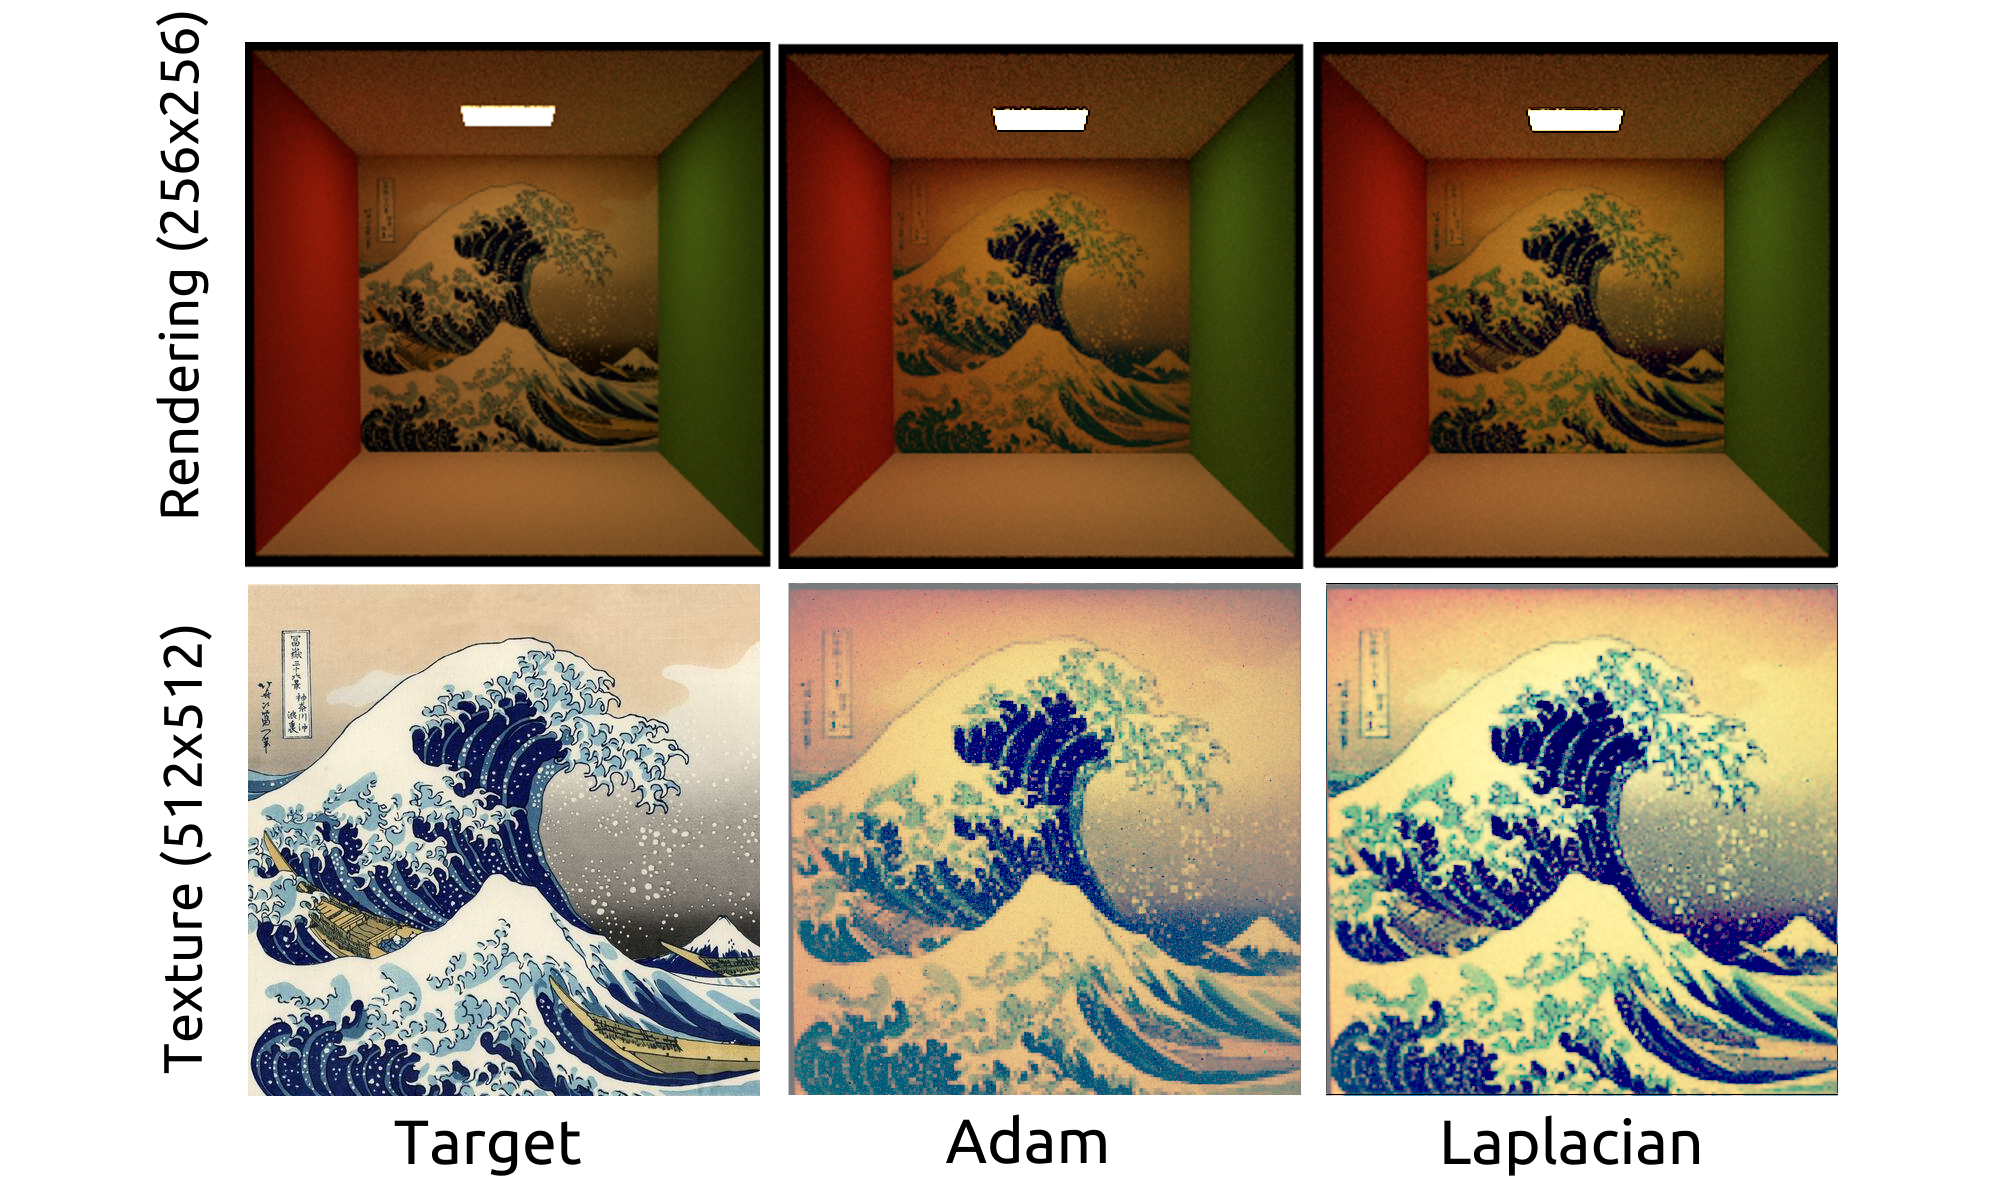
\includegraphics[width=\textwidth]{figures/result-1.png}
    \caption{Comparison of \emph{large steps} texture optimization}
    \label{fig:a-texture-comparision-Laplacian}
\end{figure}

\begin{table}[!h]
	\centering
	\resizebox{\textwidth}{!}{
	\begin{tabular}{ | c | c | c | c | c | c | c | c | c | c | c | c } \hline
		iter      & 1      & 2      & 3      & 4      & 5      & 6      & 7      & 8      & 9      & 10     \\\hline
		Adam      & 0.1433 & 0.1229 & 0.1060 & 0.0920 & 0.0808 & 0.0718 & 0.0647 & 0.0593 & 0.0554 & 0.0525 \\ \hline  
		Laplacian & 0.1433 & 0.1168 & 0.09453 & 0.0767 & 0.0627 & 0.0526 & 0.0456 & 0.0414 & 0.0394 & 0.0386 \\ \hline
	\end{tabular}}
	\caption{Comparison of \emph{large steps} texture optimization}
	\label{table:a-texture-comparision-Laplacian}
\end{table}

\subsubsection{2. Joint optimization for two texture (albedo texture and environment map)}

However, in the joint optimization case, the final image\ref{fig:joint-texture-comparision-Laplacian} shows an awful result. To analyze the result, we retested the optimization process for each parameter, and observed that the iterative procedure accumulated bias, when the target parameter was an environment map. Due to the artifact on environment map, the whole optimization process failed. This indicates that the same assumption as texture cannot be adapted to environment map, and as a result naive applying of \emph{large steps} to environment map is broken.

\begin{figure}[!h]
    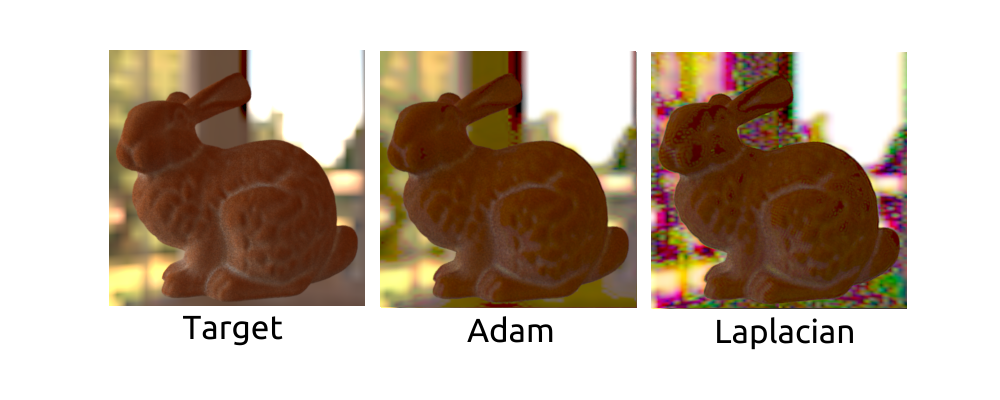
\includegraphics[width=\textwidth]{figures/result-2.png}
    \caption{Comparison of \emph{large steps} joint texture optimization: 30 iteration}
    \label{fig:joint-texture-comparision-Laplacian}
\end{figure}

\begin{figure}[!h]
    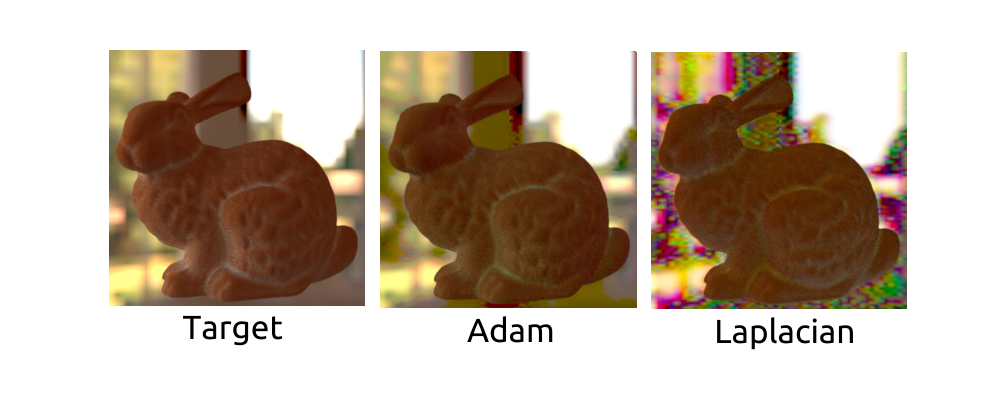
\includegraphics[width=\textwidth]{figures/result-2-1.png}
    \caption{Comparison of \emph{large steps} joint texture optimization result: only environment case}
    \label{fig:joint-texture-comparision-Laplacian-envmap}
\end{figure}

\newpage
\subsection*{Biased version: just gradient filtering}

We also test the biased version, which filters directly the gradient using gaussian blur. This implementation is really simple, just call OpenCV \emph{filter2D} function with step-size ($\lambda$) weighted gaussian kernel to texture gradients.

\subsubsection{1. A texture optimization}

Because this is biased version, there is no MSE comparison. Visually, the result\ref{fig:a-texture-comparision-gaussian} show the more clear color value. However, due to the effect of gaussian blur, the result image is more blurry than the original optimization result.

\begin{figure}[!h]
    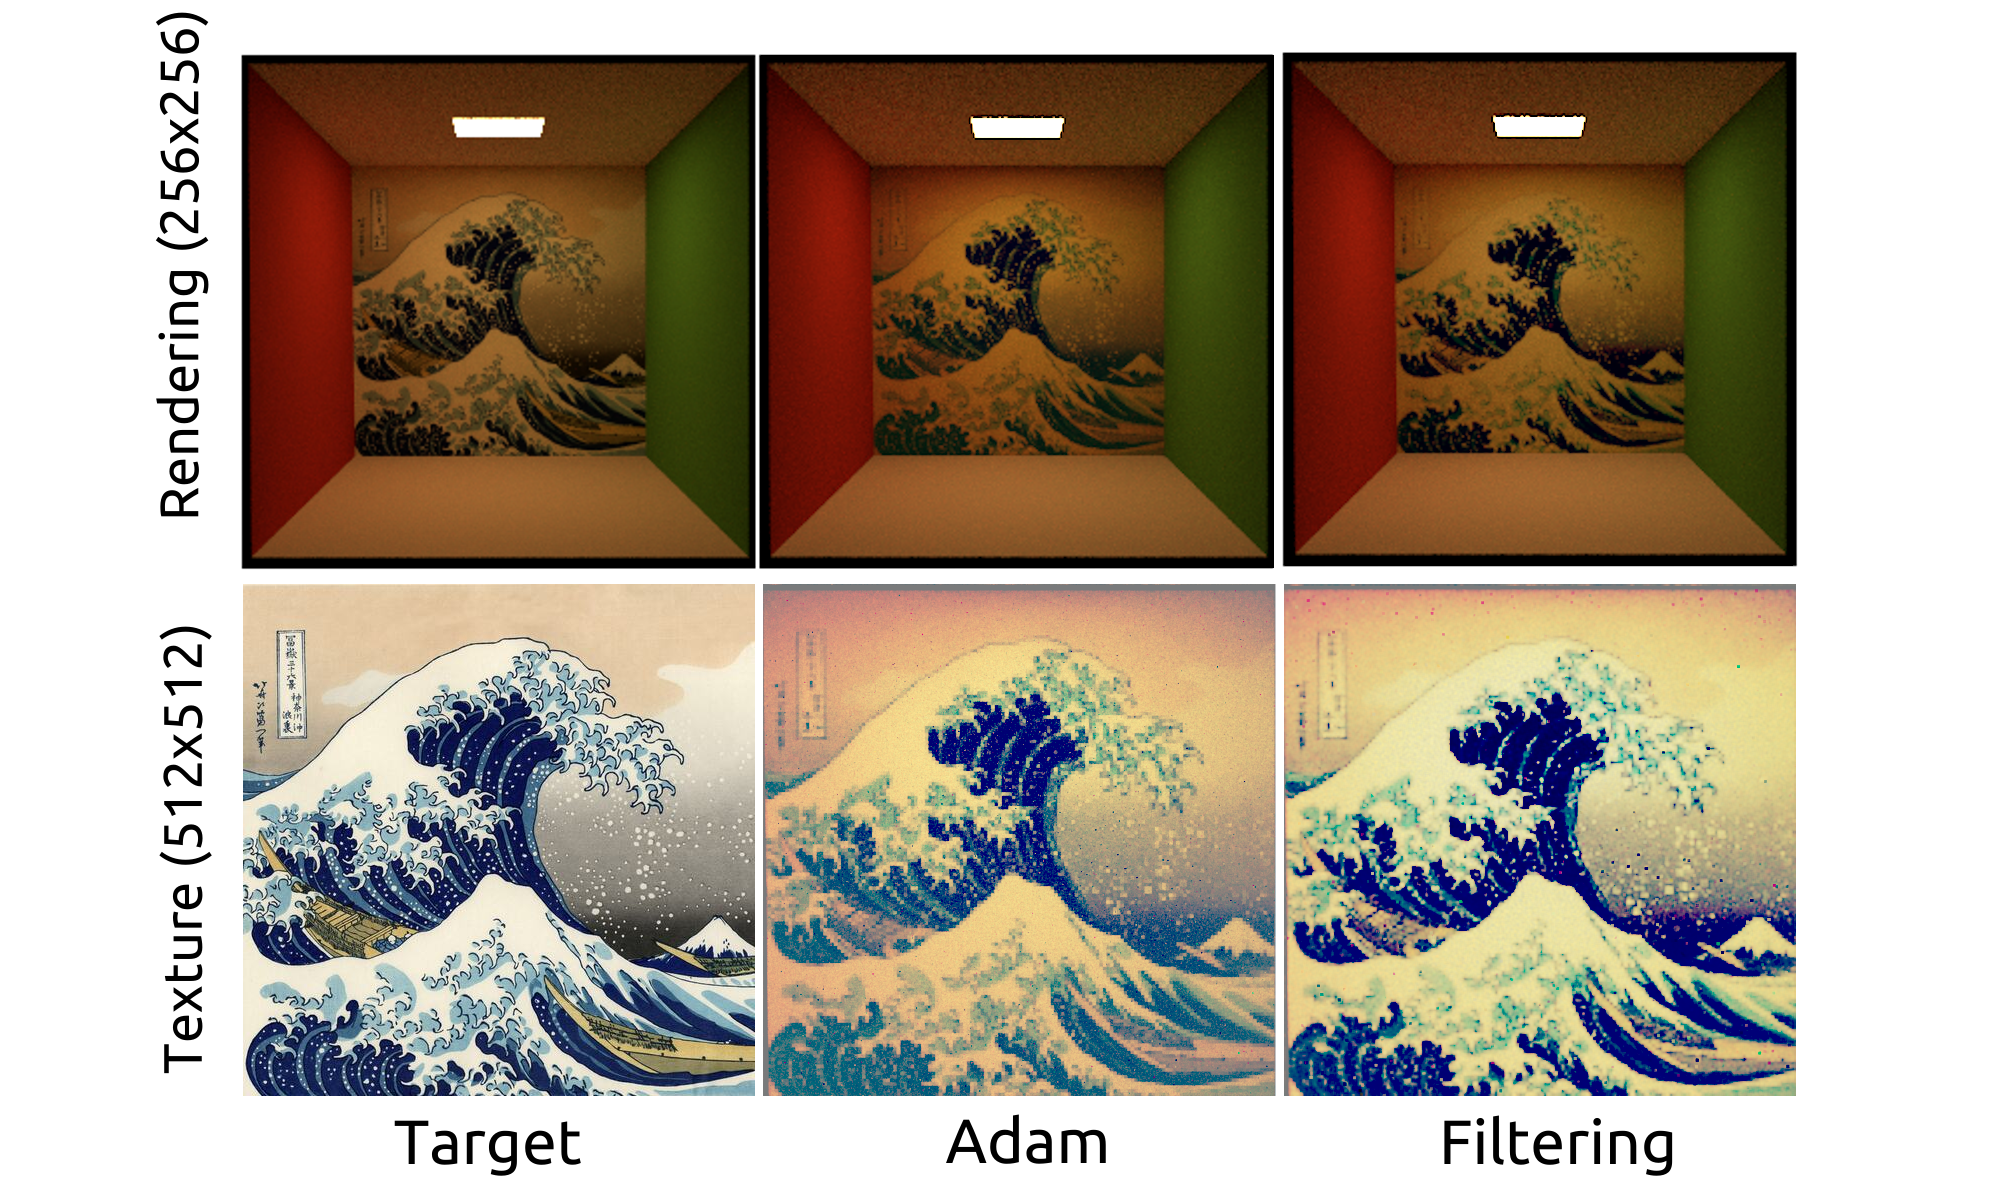
\includegraphics[width=\textwidth]{figures/result-3.png}
    \caption{Comparison of a texture optimization result}
    \label{fig:a-texture-comparision-gaussian}
\end{figure}

\subsubsection{2. Joint optimization for two texture (albedo texture and environment map)}

Moreover, in the joint optimization case of gaussian method, we can also observe the specific artifact on texture.
% more discription? 

\begin{figure}[!h]
    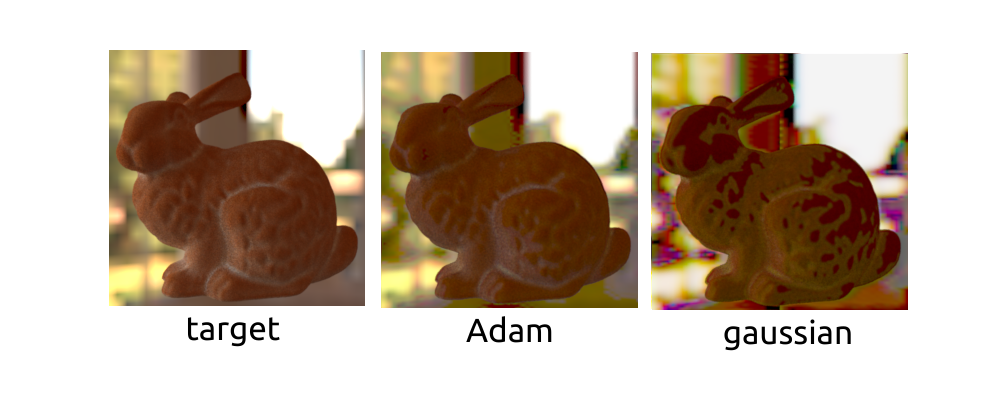
\includegraphics[width=\textwidth]{figures/result-4.png}
    \caption{Comparison of a texture optimization result: 30 iteration}
    \label{fig:a-texture-comparision-gaussian-joint}
\end{figure}